\documentclass[border=6pt]{standalone}
\usepackage{amsmath,amssymb}
\usepackage{tikz}
\usetikzlibrary{arrows.meta,shadows,calc,backgrounds}
\begin{document}
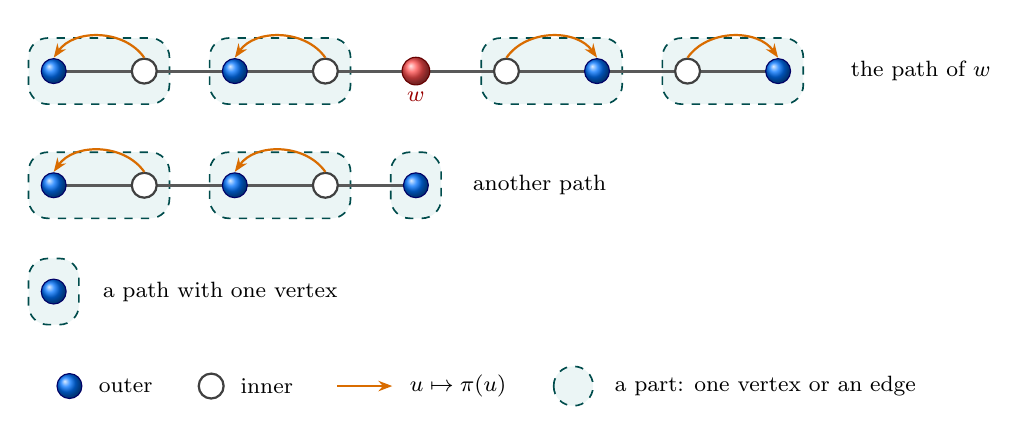
\begin{tikzpicture}[
  outer/.style={circle,inner sep=0pt,minimum size=9pt,ball color=blue!55!cyan,draw=blue!40!black,line width=0.4pt},
  inner/.style={circle,inner sep=0pt,minimum size=9pt,draw=black!75,line width=0.8pt,fill=white},
  wv/.style={circle,inner sep=0pt,minimum size=10pt,ball color=red!70,draw=red!40!black,line width=0.4pt},
  pe/.style={line width=1.1pt,black!65},
  assign/.style={-{Stealth[length=5pt]},line width=0.8pt,orange!85!black},
  part/.style={rounded corners=7pt,draw=teal!60!black,dashed,line width=0.6pt,fill=teal!8},
  lab/.style={font=\footnotesize}]
% ---------------- component of w ----------------
\foreach \i in {0,...,8} { \coordinate (a\i) at (1.15*\i,0); }
\begin{scope}[on background layer]
  \draw[part] ($(a0)+(-0.32,-0.42)$) rectangle ($(a1)+(0.32,0.42)$);
  \draw[part] ($(a2)+(-0.32,-0.42)$) rectangle ($(a3)+(0.32,0.42)$);
  \draw[part] ($(a5)+(-0.32,-0.42)$) rectangle ($(a6)+(0.32,0.42)$);
  \draw[part] ($(a7)+(-0.32,-0.42)$) rectangle ($(a8)+(0.32,0.42)$);
\end{scope}
\draw[pe] (a0) -- (a8);
\foreach \i in {0,2,6,8} { \node[outer] at (a\i) {}; }
\node[wv] (w) at (a4) {};
\foreach \i in {1,3,5,7} { \node[inner] at (a\i) {}; }
\node[lab,red!60!black,below=4pt] at (a4) {$w$};
\foreach \i/\j in {1/0,3/2} { \draw[assign] ($(a\i)+(0,0.17)$) to[bend right=55] ($(a\j)+(0,0.17)$); }
\foreach \i/\j in {5/6,7/8} { \draw[assign] ($(a\i)+(0,0.17)$) to[bend left=55] ($(a\j)+(0,0.17)$); }
\node[lab,anchor=west] at (10.0,0) {the path of $w$};
% ---------------- a second path ----------------
\foreach \i in {0,...,4} { \coordinate (b\i) at (1.15*\i,-1.45); }
\begin{scope}[on background layer]
  \draw[part] ($(b0)+(-0.32,-0.42)$) rectangle ($(b1)+(0.32,0.42)$);
  \draw[part] ($(b2)+(-0.32,-0.42)$) rectangle ($(b3)+(0.32,0.42)$);
  \draw[part] ($(b4)+(-0.32,-0.42)$) rectangle ($(b4)+(0.32,0.42)$);
\end{scope}
\draw[pe] (b0) -- (b4);
\foreach \i in {0,2,4} { \node[outer] at (b\i) {}; }
\foreach \i in {1,3} { \node[inner] at (b\i) {}; }
\foreach \i/\j in {1/0,3/2} { \draw[assign] ($(b\i)+(0,0.17)$) to[bend right=55] ($(b\j)+(0,0.17)$); }
\node[lab,anchor=west] at (5.2,-1.45) {another path};
% ---------------- an isolated vertex ----------------
\coordinate (c0) at (0,-2.8);
\begin{scope}[on background layer]
  \draw[part] ($(c0)+(-0.32,-0.42)$) rectangle ($(c0)+(0.32,0.42)$);
\end{scope}
\node[outer] at (c0) {};
\node[lab,anchor=west] at (0.5,-2.8) {a path with one vertex};
% ---------------- legend ----------------
\node[outer] at (0.2,-4.0) {}; \node[lab,anchor=west] at (0.45,-4.0) {outer};
\node[inner] at (2.0,-4.0) {}; \node[lab,anchor=west] at (2.25,-4.0) {inner};
\draw[assign] (3.6,-4.0) -- (4.3,-4.0); \node[lab,anchor=west] at (4.4,-4.0) {$u\mapsto\pi(u)$};
\draw[part] (6.35,-4.25) rectangle (6.85,-3.75); \node[lab,anchor=west] at (7.0,-4.0) {a part: one vertex or an edge};
\end{tikzpicture}
\end{document}
